\documentclass[letterpaper]{article}
\usepackage{aaai}
\usepackage{times}
\usepackage{helvet}
\usepackage{courier}
\usepackage[hyphens]{url}
\usepackage{graphicx}
\urlstyle{rm}
\def\UrlFont{\rm}
\usepackage{booktabs}
\usepackage{multirow}
\usepackage{amsmath}
\usepackage{xspace}
\frenchspacing
\setlength{\pdfpagewidth}{8.5in}
\setlength{\pdfpageheight}{11in}
\setcounter{secnumdepth}{2}

\newcommand{\carp}{\textsc{CARP}\xspace}
\newcommand{\carpcontent}{\textsc{CARP-Content}\xspace}
\newcommand{\method}{\textsc{CARP}\xspace}

\ifdefined\pdfinfo
  \pdfinfo{
  /Title (Unidentified, Yet Linkable? Measuring Provider-Side Linkage Risk in LLM Agent Traffic)
  }
\fi

\title{Unidentified, Yet Linkable?\\
Measuring Provider-Side Linkage Risk in LLM Agent Traffic}
\author{Anonymous Submission}
\nocopyright

\begin{document}
\maketitle

\begin{abstract}
Enterprise LLM gateways can strip account and session identifiers before forwarding agent requests,
creating an apparent anonymity boundary. We show that plaintext alone can undermine this boundary
for a passive provider. Recurring task objects and replayed context let otherwise unlabeled calls form
pseudonymous workflows and, when handles persist, longitudinal watchlists without identifying a person.

We define provider-side linkage risk and a controlled measurement design that separates
provider-visible traffic from linkage truth hidden from the attack. On software-engineering and
business-tool traces, paired tests perturb paths, replayed context, stable handles, and timing. These
controls isolate three channels: direct content exposure, workflow continuity, and longitudinal
propagation. We instantiate these measurements with a budgeted reference attack that links requests
and propagates stable handles.

Direct workspace and business-object handles explain the easiest recovery, but they are not the only
signals. After paths, repository slugs, and internal domains are removed, structured content links
unseen OpenHands projects at F1 0.682. On non-code traces, time-independent continuity remains at F1
0.843 after intents are rephrased. In the software traces, combining handle abstraction with non-cumulative
requests nearly eliminates session linkage, showing that the channels need separate controls.
Identifier stripping is therefore not content de-identification: agent privacy boundaries must cover
persistent task objects, replayed context, and provider log retention.
\end{abstract}

\section{Introduction}

An enterprise gateway can strip every account and session identifier from an LLM-agent call yet
still forward the content that makes the call recognizable. Paths name repositories, tool arguments
name business objects, and later turns often replay earlier messages. The calls are unidentified at
the protocol layer but may remain linkable in content.

An API broker or gateway is optional middleware between an agent and a model provider; it can
authenticate callers, route models, meter usage, and keep local state. In \emph{protocol-level
identifier stripping}, it keeps end-customer account, organization, trace, and session IDs local;
the provider authenticates the broker but receives no underlying caller mapping. Plaintext messages,
tool schemas, and outputs still pass for inference. Direct agent-to-provider deployments skip this
step and may expose still more protocol identifiers. We study the residual risk in the more protective
brokered setting.

Agent traffic makes the gap consequential. Repeated repository namespaces in code agents and
account, order, queue, or tenant objects in tool agents act as quasi-identifiers. Harm does not require
a civil identity: a stable pseudonymous cluster combines otherwise separated fragments into a
longitudinal view of co-evolving repositories and services, dependencies, failures, and migrations.
This exposes product direction, operational relationships, and security architecture as commercial
or security intelligence, while a watchlist makes the observation repeatable.

Across domains, two mechanisms produce this view: \emph{persistent content handles} retain a
namespace or object, while \emph{context replay} retransmits prior messages or state. Paired controls
must separate them because removing one does not test the other.

Prior privacy attacks recover training examples, membership, or attributes from learned models
\cite{shokri2017membership,carlini2021extracting}. Record linkage, fingerprinting, and modern
unsupervised text attribution show that removing direct identifiers need not prevent association
\cite{fellegi1969theory,sweeney2002kanonymity,narayanan2009anonymizing,eckersley2010unique,bertocco2023unsupervised}.
Our setting differs in three ways. The observer is the legitimate model API provider, and the input
is normal inference traffic rather than a released table. The output is a set of pseudonymous
cross-request partitions rather than the civil identity of a known individual.

The central measurement challenge is attribution: successful linkage may reflect a directly readable
field, retransmitted history, semantic continuity, or a stable object recurring across workflows. We
therefore ask:

\begin{quote}
Which linkage channels remain after protocol identifier stripping, under what transformations do
they survive, and can a provider measure them under a bounded candidate budget?
\end{quote}

We make three contributions:
\begin{itemize}
    \item We identify provider-side linkage as a distinct privacy failure of protocol identifier
    stripping and decompose it into direct exposure, workflow continuity, and longitudinal propagation.
    \item We develop a controlled measurement protocol that separates provider-visible traffic from
    linkage truth and uses paired removal, rephrasing, concurrency, rotation, and collision tests to
    attribute risk. These controls reveal persistent content handles and context replay as cross-domain
    root mechanisms.
    \item We instantiate the protocol with \emph{Cache-Anchored Rarity Percolation} (\textsc{CARP}),
    a budgeted reference attack. Across code and business-tool traces, we quantify residual content
    linkage, transfer, stability-dependent watchlists, partial profiling, uncertainty, and cost.
\end{itemize}

\section{Threat Model and Problem}

\subsection{Parties and Visibility}

The request flow is agent $\rightarrow$ broker $\rightarrow$ model provider. The broker may know
local identities but is not the attacker; the honest-but-curious provider sees only the forwarded
payload after the transformation above. Table~\ref{tab:assumptions} states its capabilities. The
provider is cold-start: it has no target registry or labeled history, but may derive a pseudonymous
watchlist from earlier traffic. We exclude active manipulation, broker compromise, unavailable
network metadata, and attempts to identify real natural persons.

The provider still observes the broker's upstream account, connection, and request metadata. It
cannot observe the broker's \emph{end-customer mapping} when the broker terminates the client
connection, creates a new upstream request under its own credential, and omits or remaps local
caller fields. Upstream metadata then identifies the broker, not the customer behind a call. A
pass-through gateway that forwards those fields already exposes protocol linkage and falls outside
our residual-content question.

\begin{table}[h]
\centering
\small
\begin{tabular}{@{}p{0.68\columnwidth}c@{}}
\toprule
Signal or capability & Assumed \\
\midrule
Plaintext messages and tool outputs & Yes \\
Broker account; model/time/token/tool metadata & Yes \\
Cache-like metadata & Optional \\
Access to broker-held user/session/project IDs & No \\
Evaluation labels or pre-known targets & No \\
Retention and offline analysis window & Conditional \\
Ability to alter prompts, responses, or tools & No \\
\bottomrule
\end{tabular}
\caption{Provider threat assumptions. ``Conditional'' denotes deployments that retain plaintext
long enough for offline analysis.}
\label{tab:assumptions}
\end{table}

We separate provider-only \texttt{attack\_view.jsonl} from held-out
\texttt{ground\_truth.jsonl}. Test-instance decisions read only the attack view; disjoint
development labels select reported calibration settings, and held-out truth is used only for scoring.

This visibility contract occurs in configurable services. Cloudflare AI Gateway documents
default logs containing prompts and responses, with per-request payload suppression
\cite{cloudflare2026gatewaylogs}. OpenAI documents customer-content abuse logs retained up to 30
days by default and separately approved zero-data-retention controls
\cite{openai2026datacontrols}; Microsoft likewise distinguishes prompt processing, stateful
storage, and modified abuse monitoring \cite{microsoft2026foundryprivacy}. Our threat applies to
retained-plaintext configurations, not zero-retention ones.

\subsection{Reconstruction Tasks}

Table~\ref{tab:terms} fixes the operational vocabulary used throughout the paper.

\begin{table}[h]
\centering
\footnotesize
\setlength{\tabcolsep}{3pt}
\begin{tabular}{@{}p{0.21\columnwidth}p{0.24\columnwidth}p{0.21\columnwidth}p{0.24\columnwidth}@{}}
\toprule
Term & Meaning & Term & Meaning \tabularnewline
\midrule
\raggedright Linkage & \raggedright Associate requests by workflow or task entity. & \raggedright Direct exposure & \raggedright Read a canonical label from one request. \tabularnewline
\raggedright Continuity & \raggedright Partition requests from one workflow. & \raggedright Propagation & \raggedright Assign later traffic to an earlier component. \tabularnewline
\raggedright Profiling & \raggedright Aggregate supported component attributes. & \raggedright Watchlist & \raggedright Earlier components retained for later matching. \tabularnewline
\bottomrule
\end{tabular}
\caption{Operational terms. Outputs are pseudonymous; none implies natural-person identification.}
\label{tab:terms}
\end{table}

The common evaluation slots---session, user/customer-like, project/process, and tenant/owner-like---
are dataset-specific interfaces, not a universal enterprise hierarchy. Open-SWE project/owner
denotes repository/GitHub-owner truth, whereas the controlled tau-bench overlay supplies customer,
project, and tenant entities.

We evaluate linkage using pairwise precision, recall, and F1, together with purity and cluster
counts. For project and organization levels, we additionally exclude all request pairs from the
same workflow; this cross-workflow metric tests longer-lived association without credit for merely
grouping turns of one session. We separately evaluate turn ordering, longitudinal assignment, and
field-level profile precision/recall/F1. Bootstrap units follow the natural hierarchy: workflows
for cold-start linkage, entities for watchlists, and organizations for profile reconstruction.

\paragraph{Measurement requirements.}
Provider traffic is nested, streaming, multi-level, and initially unlabeled. A valid measurement
must separate provider-visible input from truth, prevent within-workflow evidence from inflating
longer-lived entity scores, evaluate watchlists only on later traffic, and bound candidate generation.
\carp is our reference instantiation of these requirements.

\section{Measurement Design and Reference Attack}

\begin{figure*}[t]
    \centering
    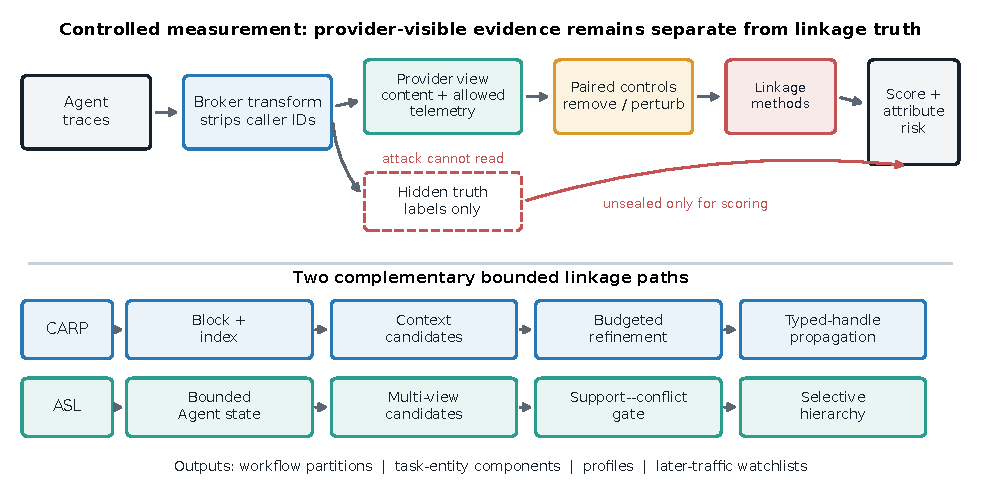
\includegraphics[width=0.98\textwidth]{figures/carp_pipeline.pdf}
    \caption{Measurement framework and reference attack. The upper lane enforces the threat
    contract: paired controls alter only the provider-visible attack view, attacks cannot read the
    sealed truth, and labels are unsealed only for scoring. The lower lane instantiates the attack
    with \carp's five bounded sparse-linkage steps.}
    \label{fig:carp}
\end{figure*}

\subsection{Provider-Visible Evidence}

For each request, extraction is capped at 80K characters, 8K shingles, and 5K words. We retain rare
identifiers, workspace paths, repository owner/name pairs, internal domains, trace-like strings, tool
and system fingerprints, semantic signatures, request time, length, and a cache-like bucket. For
non-code traffic, a structured parser reads tool JSON and explicit ``X ID'' phrases,
typing user/email, order/reservation/queue, and tenant/domain handles by linkage level. Shared
flight/product resources remain candidate evidence, while broad region, tier, and status values are
excluded from union anchors.

\subsection{Budgeted Linkage Pipeline}

\carp maps provider-visible request streams to level-specific partitions under a per-request
candidate budget. It orders evidence from cheap local blocking to type-aware edges and finally
cross-block propagation; separate components prevent a user signal from silently becoming a project
or organization link. The outputs are predicted partitions, candidate diagnostics, and optional
later-traffic assignments. Local processing is bounded by $O(nB)$ for budget $B$; typed-anchor
propagation uses connected components rather than all-pairs request comparison. Five deterministic stages
implement this order (Figure~\ref{fig:carp}). First, cache-like metadata blocks local comparison; it
never determines a label. Missing metadata maps to one
\texttt{cache\_unavailable} block, as in Open-SWE, so cache telemetry cannot explain that result.
Second, exact inverted indexes join bounded-frequency anchors. Maximum bucket sizes are 20 for
session traces, 80 for user/customer anchors, and 400 for project and tenant/owner anchors.

Third, two bounded context passes generate session candidates. Semantic buckets contain at most 20
requests and link a pair only with at least two semantic matches, shingle Jaccard at least 0.32,
three shared identifiers, and a 90-minute gap. Shingle buckets contain at most 35 requests. They link
cumulative contexts when smaller-context containment is at least 0.78, Jaccard is at least 0.20, two
identifiers and one repository agree, and the gap is at most 180 minutes.

Fourth, refinement considers buckets of at most 20 requests, never more than 400 candidate pairs
per request. It links sessions when Jaccard is at least 0.22 with two identifiers within 180
minutes, or when Jaccard is at least 0.24 with two semantic and three identifier matches within 90
minutes. Project and tenant/owner edges require an exact
typed repository, business-object, domain, or owner overlap; user edges require either an exact
business-user anchor or a fixed 1.8 weighted threshold over username, identifier, semantic, and
time agreement. Separate union-find structures preserve the four evaluation partitions.

Finally, strong-entity percolation operates across cache blocks without all-pairs request
comparison. It builds separate components over stable user, process/project, and organization
handles. Shared resources never create direct unions; an alias that bridges multiple stronger typed
components is rejected by provider-visible co-occurrence. Numeric thresholds and pair budgets are
fixed within each reported protocol; no evaluation label is read to make a test-instance decision.

\subsection{Content Reconstruction and Longitudinal Assignment}

Within a predicted cluster, context containment and request time reconstruct the workflow sequence.
A structured profiler aggregates lexical, file-extension, manifest, command, repository, service,
and domain evidence. A dense-semantic baseline extracts at most eight technical spans per request,
retrieves a fixed ontology with all-MiniLM-L6-v2
\cite{reimers2019sentencebert,wang2020minilm}, filters negation and migration contexts, and requires
calibrated cross-request support. Every profile value retains request-level evidence.

An optional \carpcontent stage spends more computation after sparse discovery. For non-code
sessions it masks identifier values, embeds the stable initial task intent with MiniLM, retrieves 24
neighbors, and combines semantic similarity with bounded typed-object matches. For projects after
path abstraction, it aggregates each recovered session, combines structured term-frequency/
inverse-document-frequency (TF--IDF) evidence with MiniLM,
and applies a structural-similarity gate before union. Neither stage reads timestamps.

For longitudinal tracking, early predicted clusters yield an entity watchlist. Exact typed anchors
map later requests back to an earlier cluster only when the anchor is unique or wins an
unambiguous vote. Evaluation truth is used only to score these assignments.

\section{Datasets and Experimental Setup}

\paragraph{Open-SWE-Traces.}
Our main real-data substrate is the \texttt{nvidia/Open-SWE-Traces} dataset
\cite{nvidiaopenswetraces}, containing trajectories
from software-engineering agent scaffolds including OpenHands
\cite{wang2024openhands}. We convert up to 12 turns per trajectory into provider-view requests.
The main 1,000-trajectory sample supplies 12,000 requests. Reliable labels are workflow,
repository/project, and GitHub owner. We reserve a fixed 100-workflow development slice for
engineering checks and evaluate the remaining 900 workflows; turns 3, 6, 9, and 12 provide 3,600
held-out requests. We use controlled provider-view timestamps; cache telemetry and a reliable user
label are unavailable. A separate 500-workflow SWE-agent sample supports cross-scaffold evaluation.

\paragraph{tau-bench historical.}
tau-bench contains airline and retail tool-agent trajectories
\cite{yao2024taubench}. We convert each assistant turn and its cumulative preceding dialogue/tool
state into a provider-view request. A 200-workflow reservoir contains 2,175 requests. We reserve a
domain-stratified deterministic 40-workflow calibration split and evaluate the remaining 160
workflows (1,736 requests); the stable-handle parser itself is deterministic and uncalibrated.

\paragraph{Trace-grounded overlays.}
Two Open-SWE overlays inject controlled user/environment/profile signals into real traces, either
retaining distinguishable user signals or intentionally sharing them. A controlled tau-bench entity
overlay, denoted T3, places 24 synthetic tenants, 140 customers, and 72 business projects over 660
real trajectories, producing 7,099 time-mixed requests and controlled hierarchical truth.

\paragraph{Baselines and controls.}
We compare temporal buckets, tool/system fingerprints, rare-anchor linkage, prefix/shingle
linkage, and \carp. A high-fidelity Hybrid diagnostic uses larger exact-anchor buckets and
multifeature pair rules. A bounded context-only diagnostic removes rare, semantic, and entity
propagation. A repository-anchor control uses only the normalized
repository and owner components parsed from OpenHands workspace paths. Random and oracle-size
random partitions are negative controls. Feature
ablations remove paths, repository identifiers, shingles, semantic signatures, tool schema, or
cumulative context.

\paragraph{Data separation.}
The main Open-SWE view fixes turns 3, 6, 9, and 12 for every trajectory. Every method receives the
same 3,600 held-out requests; the 100-workflow development slice is excluded from the main metrics.
This controls repeated-turn count and keeps cumulative feature extraction tractable, while the
full 10,800-request held-out set (900 workflows, up to 12 turns) is used only for the direct-exposure
audit. The 12,000-request source remains the basis for longitudinal and trace-grounded cost runs.

\paragraph{Calibration and uncertainty.}
The main \carp linkage run disables optional semantic signatures; the development-slice semantic
ablation leaves its scores unchanged. Open-SWE local-link thresholds and budgets are checked once
on the development slice and then frozen for the 900-workflow evaluation. T3 fixes its typed anchor
vocabulary and ambiguity rule on the first 2,500 requests before evaluating later traffic. The
profile MiniLM baseline selects its retrieval threshold and minimum support on 124 owner-like
calibration groups, then evaluates 432
disjoint groups. The default historical tau-bench \carp row transfers the shared thresholds without
retuning. A separate high-precision point selects the maximum-F1 semantic-signature setting with
calibration precision at least 0.8 over a fixed threshold grid. The selected rule requires four
semantic matches, shingle Jaccard 0.32, three identifiers, and a 30-minute gap. We report temporal,
tool, context, hybrid, random, and \carp baselines on 160 held-out workflows, including
airline/retail breakdowns. Open-SWE and historical tau-bench confidence intervals (CIs) use 200
workflow resamples; T3 and profile-extension intervals use 500
resamples, all with seed 7.

\paragraph{Paired transformations.}
For temporal stress, we preserve within-workflow order but compress arrivals from the converted
five-minute spacing to 60 or 15 seconds. Adding up to two or five minutes of deterministic jitter
raises peak active workflows from 2 to 10 or 41. \carpcontent selects cosine threshold 0.98 on the 40
calibration workflows. A separate lexical-rephrasing stress changes each retransmitted task form.
The strict Open-SWE project stage uses a project-disjoint 25/75 split: 160 projects calibrate its
TF--IDF/MiniLM threshold and 479 unseen projects are evaluated.

For strict Open-SWE removal, we rewrite provider-visible content to remove workspace/home paths,
repository fields and slugs, and internal domains before feature extraction. This diagnostic uses
24K characters, 1,200 shingles, and 1,500 words per request. T3 stress tests independently vary
anchor occurrence retention, later-traffic alias rotation, and shared-anchor collision.

\paragraph{Artifact availability.}
The anonymized artifact includes code, locked dependencies, configs, attack-view generators,
random seeds, derived tables, and figure scripts; redistribution of raw benchmark text remains
subject to upstream licenses.

\section{Results}

\begin{table}[h]
\centering
\footnotesize
\begin{tabular}{@{}p{0.22\columnwidth}p{0.72\columnwidth}@{}}
\toprule
Channel & What the decisive controls establish \tabularnewline
\midrule
\raggedright Task objects & \raggedright Repo-only F1 .994/.981 and strict direct F1 0 identify explicit exposure; residual .682 and cross-scaffold .318 show partial non-path signal. \tabularnewline
\raggedright Continuity & \raggedright Replay explains exact recovery; after removing it, rephrased content still gives time-independent F1 .843. \tabularnewline
\raggedright Propagation & \raggedright Natural later-alias F1 .984 and zero under T3 rotation tie tracking to stable handle lifecycles. \tabularnewline
\raggedright Profile/cost & \raggedright Profile F1 .809 and 11.2 pairs/request at 100K show bounded partial reconstruction. \tabularnewline
\bottomrule
\end{tabular}
\caption{Overall takeaways from the decisive controls.}
\label{tab:takeaways}
\end{table}

\subsection{RQ1: What Does Identifier Stripping Leave Exposed?}

In the 10,800-request direct audit, every request contains a parser-recoverable canonical repository
and owner-like label. Project anchors are multi-valued in 5.5\% of requests but always include the
canonical label; owner anchors are unambiguous. These are sanitization failures, not hidden inference.

\begin{table}[t]
\centering
\small
\begin{tabular}{@{}lrrr@{}}
\toprule
Setting & Sess. & Project & Owner \\
\midrule
Exact nesting & 1.000 & --- & --- \\
Hybrid & .983 & .994 & .981 \\
\carp & .967 & .994 & .981 \\
Repo/owner only & --- & .994 & .981 \\
\carp, turn delta & .117 & --- & --- \\
Strict, cumulative & .183 & .000 & .000 \\
Strict, turn delta & .016 & .000 & .000 \\
\bottomrule
\end{tabular}
\caption{Attack-surface matrix on 3,600 held-out Open-SWE requests. Exact nesting diagnoses
message-prefix exposure; project/owner columns exclude within-workflow pairs. Strict rows rewrite
paths, repository strings, and internal domains.}
\label{tab:openswe}
\end{table}

Hybrid, \carp, and the repository-anchor control are identical on the held-out slice:
cross-workflow project/owner F1 is 0.994 ([0.977,1.000]) and 0.981 ([0.956,0.996]). The scores
therefore come from explicit OpenHands path components, not a \carp gain over exact anchors;
SWE-agent lacks this representation and yields zero.

Path abstraction does not end the analysis. After exact nesting first recovers sanitized sessions,
\carpcontent links 764 sessions from 479 project identities unseen during calibration using residual
task, code, test, and tool evidence. It reaches project precision/recall/F1 0.795/0.597/0.682,
with entity-bootstrap F1 CI [0.578,0.772], whereas the strict direct-anchor stage is zero;
dense-only F1 is 0.070. Thus explicit paths dominate
the first stage, but structured non-path evidence supports partial second-stage association.
With target-specific calibration, the same strict protocol reaches precision/recall/F1
0.942/0.286/0.439 on 280 unseen SWE-agent projects. For genuine zero-target-label transfer, we
freeze source-selected feature weights and use mutual-nearest edges with a source-selected ambiguity
margin. OpenHands$\rightarrow$SWE-agent reaches 0.909/0.193/0.318 (F1 CI [0.247,0.439]); the reverse
direction reaches 0.978/0.098/0.179 ([0.119,0.252]). Absolute thresholds collapse under domain
shift, whereas mutual agreement preserves high precision at a recall cost.

\subsection{RQ2: How Much Workflow Continuity Remains?}

Exact cumulative-prefix matching recovers every held-out Open-SWE workflow at F1 1.000, versus
Hybrid 0.983 and bounded \carp 0.967; the paired \carp-minus-Hybrid interval is
$[-0.039,-0.002]$. On turn-delta requests both fall to 0.117 ([0.105,0.130]); adding strict content
removal eliminates project/owner linkage and lowers session F1 to 0.016. Exact nesting remains
1.000 on strictly sanitized cumulative requests, isolating retransmitted dialogue from entity handles.

On 160 held-out historical tau-bench workflows, 10-minute grouping reaches
precision/recall/F1 0.702/0.774/0.736 (F1 CI [0.674,0.807]), while default \carp reaches F1 0.495.
This advantage is schedule-induced: at peak concurrency 10/41/146, temporal F1 falls to
0.125/0.035/0.013 and default \carp to about 0.021. Time-independent \carpcontent instead reaches
precision/recall/F1 0.922/1.000/0.960 and is invariant to those timestamp transformations. An exact
normalized-intent hash reaches 1.000 because cumulative requests retransmit the same initial task.
When each request receives a deterministic lexical rephrasing, that hash falls to F1 0.309 while
\carpcontent retains precision/recall/F1 0.944/0.762/0.843 (CI [0.791,0.878]). The expensive semantic stage is thus
unnecessary for verbatim repetition but useful when surface form changes.

\subsection{RQ3: Do Stable Anchors Enable Longitudinal Propagation?}

Natural tau traces first establish that persistence is not solely an overlay artifact. On the
160-workflow holdout,
parsing tool JSON and explicit ID phrases covers 62.8\% of requests and links benchmark-user traffic
at precision/recall/F1 1.000/0.400/0.571 (CI [0.515,0.623]); cross-workflow F1 is 0.561.
User-ID-only and email-only F1 are 0.473/0.491, while removing stable handles gives zero. In a
separate 100/100 longitudinal split, removing later user IDs but retaining email/name--zip aliases
gives F1 0.984 (CI [0.959,1.000]); name--zip alone gives 0.624. Thus stable content handles recur
across non-code workflows without injected T3 entities.

T3 then isolates how cross-cache propagation and handle stability affect coverage.
Figure~\ref{fig:t3} summarizes the result: percolation raises user/project/tenant F1 from
0.214/0.159/0.297 to 0.771/0.686/0.777. Precision is 0.952/0.998/1.000 and recall is
0.648/0.522/0.635; paired F1-gain intervals are [0.522,0.590], [0.498,0.553], and
[0.461,0.497].

An entity watchlist built from the first 2,500 requests is evaluated only on later traffic. It
reaches user/project/tenant F1 0.702/0.830/0.876. Entity-bootstrap 95\% intervals are
[0.675,0.725], [0.816,0.840], and [0.860,0.891]. In the controlled configuration,
customer/project/tenant anchor coverage is 0.576/0.718/0.800, median observed lifetimes are roughly
13--19 days, and only account-cache anchors show ambiguity (3.7\%). At 50\% occurrence retention,
watchlist F1 falls to 0.578/0.681/0.630; rotating every later alias reduces all three to zero. With
25\% shared-anchor collision, conservative ambiguity rejection keeps precision
0.926/1.000/1.000 but lowers F1 to 0.691/0.753/0.800. The rotation and collision curves directly
quantify how longitudinal propagation depends on anchor stability.

\begin{figure}[t]
    \centering
    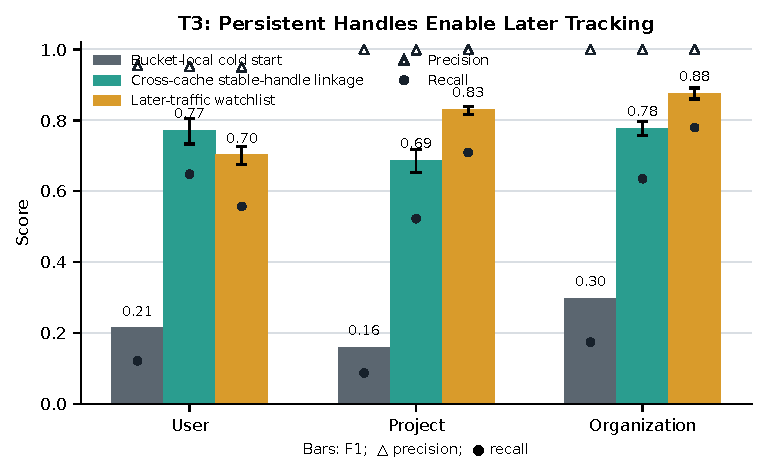
\includegraphics[width=\columnwidth]{figures/t3_longitudinal.pdf}
    \caption{T3 F1 bars with 95\% intervals; triangles/circles mark precision/recall. T3 uses
    trace-grounded semi-synthetic entity truth.}
    \label{fig:t3}
\end{figure}

\paragraph{Partial technical profiling.}

Structured evidence raises fixed-ontology technical-field F1 from 0.623 to 0.809; using truth clusters
changes it only to 0.812. On 432 unseen owner-like groups, structured and MiniLM profilers both
round to 0.807, while four artifact-supported MiniLM predictions are absent from fixed truth. This
supports partial technical reconstruction and reveals a fixed-truth coverage limit.

\subsection{RQ4: Can Risk Be Measured Under Bounded Pair Budgets?}

Bounded candidates, rather than exhaustive pairs, determine \carp's cost. For the two 12,000-request
Open-SWE overlays, all-pairs comparison requires 71,994,000 pairs; streamed \carp considers
361,997/366,211 respectively, a 197--199$\times$ reduction. Single-machine time is 291/233 seconds with peak
resident set size (RSS) 1.30/1.37 GB. MiniLM embeds 21,507 post-discovery spans in 107 seconds at
2.27 GB peak RSS.

A controlled scale diagnostic grows from 10K to 50K and 100K requests while holding
four requests/workflow, bucket occupancy, and collision rate fixed. Pair comparisons remain
11.0/request without collisions and 11.2 with shared-alias collisions; true-session candidate recall
is 1.000. Linkage time is 2.1/11.0/23.1 seconds and peak RSS 0.10/0.35/0.66 GB. Collision-stress
precision/recall/F1 remains 0.882/1.000/0.938 across all sizes, while exhaustive-pair reduction
grows from 446$\times$ to 4,464$\times$.

On the held-out Open-SWE fixed-turn diagnostic with scale caps, the union of \carp's candidate sets
contains 31,473 pairs. It retains all 5,400 true session pairs (candidate recall 1.000, precision
0.172), so its accuracy loss is downstream of blocking. A 32-value bottom-$k$ shingle sketch,
matched in eight bands of
four, retains 46,087 candidates with recall 0.990 and reaches session F1 0.858. This control places
\carp's sparse retrieval against an approximate-nearest-neighbor (ANN) alternative at matched scale.

On the same held-out set, a post hoc context-stage sensitivity sweep retains candidate recall 1.000
for pair budgets 100--800. F1 stays 0.910 across those budgets and Jaccard 0.16--0.24. It changes
from 0.981 to 0.572 as containment rises from 0.62 to 0.94, making containment the only materially
sensitive parameter in this sweep.

We additionally index the 1,736 held-out tau-bench intent embeddings with a standard hierarchical
navigable small-world (HNSW) index \cite{malkov2020hnsw}. At
\texttt{efSearch}=200 it retains 0.993 of true session pairs and reaches F1 0.956, versus 0.960 for
exact dense top-$k$; index build/query time is 0.24/0.09 seconds. Thus a standard ANN backend
preserves almost all candidate recall and final linkage accuracy.

\subsection{Mitigation Implications}

The controls require both persistent-handle minimization and non-cumulative context: strict path
removal drives project/owner F1 to zero but leaves cumulative session F1 0.183, whereas combining
the two reaches 0.016 from 0.967. This motivates unstable namespaces, typed-object minimization,
shorter retained context, and provider log governance.

\section{Related Work}

\paragraph{Record linkage, matching, and attribution.}
Statistical record linkage formalizes noisy matching \cite{fellegi1969theory}; modern systems combine
blocking and filtering with learned matchers
\cite{christen2012survey,papadakis2020blocking,li2020ditto}, and recent benchmarks quantify their
candidate-quality tradeoffs \cite{neuhof2024benchmark}. Collective entity resolution propagates
relational evidence \cite{bhattacharya2007collective}. \carp adopts these established primitives but
targets a stream of nested agent requests with separate session and task-entity outputs.
Quasi-identifiers, graph and website de-anonymization, and author identification show why deleting
names does not guarantee unlinkability
\cite{sweeney2002kanonymity,narayanan2009anonymizing,panchenko2016website,narayanan2012author}.
Recent unsupervised attribution and LLM-based authorship-privacy studies extend that lesson to modern
text representations \cite{bertocco2023unsupervised,nguyen2025authorship}. Our output is instead a
pseudonymous partition with no target registry.

\paragraph{Language-model privacy.}
Membership inference and training-data extraction target information encoded in model parameters
\cite{shokri2017membership,carlini2021extracting}; LLMs can also infer sensitive attributes from
otherwise ordinary text \cite{staab2024beyond}, and text embeddings can be inverted to recover much
of their source content \cite{morris2023embeddings}. By contrast, recent text anonymization rewrites
content while explicitly balancing privacy and utility \cite{yang2025anonymization}. Identifier
stripping is a weaker transformation. Our provider already sees plaintext inference inputs: the
failure is cross-request association followed by evidence accumulation, not model memorization or
embedding inversion. Differential privacy offers a training-time guarantee
\cite{dwork2006calibrating} but does not hide tool context supplied at inference time.

\paragraph{Agent evaluation and security.}
SWE-bench and OpenHands evaluate software problem solving and agent interfaces
\cite{jimenez2023swebench,wang2024openhands}. tau-bench evaluates tool-agent-user interaction
\cite{yao2024taubench}. Prompt-injection work shows that tool-integrated applications enlarge the
attack surface \cite{greshake2023indirect,debenedetti2024agentdojo,yi2025promptinjection}. These works
primarily study
task success or active compromise. We study a passive provider that links otherwise normal agent
traffic.

\section{Ethics, Scope, and Limitations}

Our evidence uses public benchmark traces and controlled overlays rather than production provider
logs or natural-person identities. Open-SWE labels denote repositories and GitHub owners,
historical tau labels denote benchmark user records, and controlled anchors may differ from deployed
business objects; the 100K experiment measures computational scaling rather than production
prevalence. The offline threat requires retained plaintext and authorized access, while zero-retention,
encryption, law, and policy constrain its applicability. Released examples remain redacted and
aggregated.

\section{Conclusion}

Removing IDs does not remove links. Protocol identifier stripping leaves three separable risks.
Persistent namespace and business-object handles expose longer-lived associations, while cumulative
prefixes expose workflow continuity. Even after paths and namespaces are removed, structured content
supports partial project linkage and rephrased-intent continuity; when handles persist, their stability
determines watchlist reach.
Conversely, strict path abstraction plus non-cumulative requests reduces session F1 from 0.967 to
0.016, showing that the channels require distinct controls. Together, these measurements locate the
residual channels and show that they can be tested under bounded candidate budgets. Agent privacy
architectures must distinguish metadata stripping from content minimization and include retransmitted
context and stable task objects in the identity boundary\label{paper:body-end}.

\bibliography{references}
\bibliographystyle{aaai}

\end{document}
